\documentclass[aspectratio=169, xetex, 12pt]{beamer}
\usepackage[utf8]{inputenc}
\usepackage[T1]{fontenc}
\usepackage{datetime}

\usetheme[mode=dark]{extia}
\title{Les nouveautés de Python 3.11}
\author{Clément Dubos}
\institute{Extia}
\newdate{date}{06}{09}{2022}
\date{\displaydate{date}}

\begin{document}

    \maketitle

    \begin{frame}{Sommaire}
        \hfill
        \parbox[t]{.9\textwidth}{
            \begin{minipage}[c][0.2\textheight]{\textwidth}
                \Large
                \tableofcontents
            \end{minipage}
        }
    \end{frame}

    \section{Optimization and Performance}

    \begin{frame}{Faster CPython}{Generalité}
        \begin{minipage}[t]{0.5\paperwidth}
            \begin{block}{Faster CPython, un projet ambitieux}
                \begin{itemize}
                    \item Initiative: Microsoft et Guido Van Rossum
                    \item Objectif: \textbf{x5} en 2025 => 1.5/an
                    \item basé sur \textbf{HotPy} et \textbf{HotPy2}
                    \item Incrémental sur les différentes version de python a venir.
                \end{itemize}
            \end{block}
        \end{minipage}
        \hspace{.1cm}
        \begin{minipage}[t]{0.4\paperwidth}
            \begin{block}{Statut actuel}
                \begin{itemize}
                    \item Speedup \textbf{x1.25} en moyenne
                    \item Entre \textbf{x1.10} et \textbf{x1.60} selon le workload
                    \item \href{https://docs.python.org/3.11/whatsnew/3.11.html\#faster-cpython}{Python 3.11 Faster Cpython}
                \end{itemize}
            \end{block}
        \end{minipage}
    \end{frame}

    \begin{frame}{Faster CPython}{Détail - Startup}

        \begin{block}{Speedup du démarrage}
            \begin{itemize}
                \item code object et bytecode statiquement alloué par l'interpréteur
                pour les modules essentiels aux démarrage
            \end{itemize}
        \end{block}
        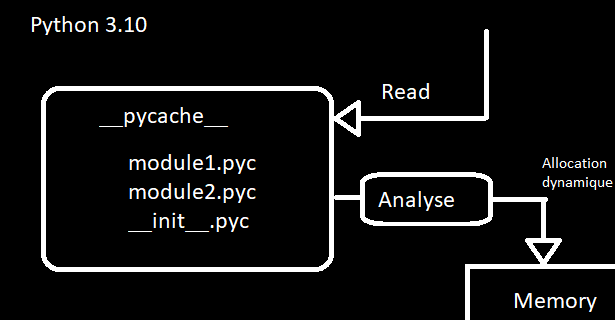
\includegraphics[scale=0.4]{img/workflow_startup310.png}
        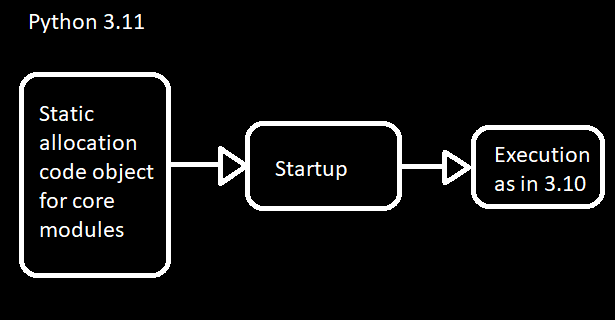
\includegraphics[scale=0.4]{img/workflow_startup311.png}
    \end{frame}

    \begin{frame}{Faster CPython}{Détail - Runtime}
        \begin{block}{Speedup du runtime}
            \begin{itemize}
                \item Reduction de l'information d'execution en memoire (debug ou on-demand). \textbf{3-7\%}
                \item mechanisme de "jump" lors d'un appel de function (skip function d'interpretation C). \textbf{1-3\%}
                \item \href{https://github.com/brandtbucher/specialist}{Specializing Adaptive Interpreter}
            \end{itemize}
        \end{block}
        \begin{block}{Misc}
            \begin{itemize}
                \item les objets nécessite moins d'espace mémoire
                \item Représentation des exceptions plus concise, améliore le catchin de \textbf{10\%}
            \end{itemize}
        \end{block}
    \end{frame}

    \begin{frame}{Optimisation Global}
        \begin{block}{Optimisation}
            \begin{itemize}
                \item C-style formatting \textbf{\%s}, \textbf{\%r}, \textbf{\%a} est maintenant aussi efficace que les f-string
                \item "Zero-cost" exception => cout du \textbf{try} casi null lorsqu'il n'y a pas d'exception
                \item Les \textbf{dict} ne stock plus les \textbf{hash} lorsqu'il ne manipule que des objet unicode => reduction espace mémoire
                \item module \textbf{re} refactorisé en partie, \textbf{10\%} plus rapide.
            \end{itemize}
        \end{block}
    \end{frame}

    \section{Exceptions}
    \begin{frame}{Exceptions}
        \begin{block}{Exception Groups and except*}
            \begin{itemize}
                \item \href{https://peps.python.org/pep-0654/}{PEP 654}
            \end{itemize}
        \end{block}
        \begin{block}{Enriching Exceptions with Notes}
            \begin{itemize}
                \item ajout d'une methode \textbf{add\_note} pour les exceptions
            \end{itemize}
        \end{block}
        \begin{block}{Improved Error Locations in Tracebacks}
            \begin{itemize}
                \item \href{https://docs.python.org/3.11/whatsnew/3.11.html\#enhanced-error-locations-in-tracebacks}{Error Locations in Tracebacks Exemple}
            \end{itemize}
        \end{block}
    \end{frame}

    \section{Typing improvements}
    \begin{frame}{Typing improvements}{Part - 1}
        \begin{block}{Variadic generics}
            \begin{itemize}
                \item Introduit \textbf{TypeVarTuple} pour les Variadic Generic
                \item Variadic Generic: Nombre variable d'entrée de type variable
            \end{itemize}
        \end{block}
        \begin{block}{Self type}
            \begin{itemize}
                \item Ajout de l'annotation \textbf{Self} pour les retour du type de l'objet
            \end{itemize}
        \end{block}
    \end{frame}
    \begin{frame}{Typing improvements}{Part - 2}
        \begin{block}{Individual TypedDict items}
            \begin{itemize}
                \item \textbf{TypedDict} peut marqué ses items comme \textbf{Required} ou \textbf{NotRequired}
                \item Les items sont \textbf{Required} par défaut, sauf si \textbf{total=False}
            \end{itemize}
        \end{block}
        \begin{block}{Arbitrary literal string type}
            \begin{itemize}
                \item l'annotation \textbf{LiteralString} permet de marquer une variable comme une string \textit{statique}
            \end{itemize}
        \end{block}
    \end{frame}

    \section{Major Language and Modules Changes}
    \begin{frame}{Major Language and Modules Changes}
        \begin{block}{Major Language Changes}
            \begin{itemize}
                \item * utilisable a présent dans les \textbf{for statement}
                \item \textbf{PYTHONSAFEPATH} / \textbf{-P} option pour les \textbf{path} potentiellement
                non secure pour le \textbf{sys.path}
                \item \textbf{sys.path} ne supporte plus les \textbf{Bytes}
            \end{itemize}
        \end{block}
        \begin{block}{Major Modules Updates}
            \begin{itemize}
                \item \textbf{AsyncIO} => \textbf{TaskGroup} context manager
                \item \textbf{contextlib} => \textbf{chdir} context manager
                \item \textbf{re} => atomic groups et possessive quantifier
                \item \textbf{unittest} => \textbf{enterContext()} et \textbf{enterClassContext()}
            \end{itemize}
        \end{block}
    \end{frame}

\end{document}
